\documentclass[D:/Latex/Internship/Report/Latex/Report.tex]{subfiles}
%\documentclass[C:/Users/USER/Desktop/Project/Intership/Report_Latex_example/Report/Latex/Report.tex]{subfiles}
\usepackage[utf8]{inputenc}
\PassOptionsToPackage{english, british}{babel}
\usepackage[english, british]{babel}
\usepackage{graphicx}
\usepackage{setspace}
\graphicspath{{Figure/}}


\begin{document}
	\begin{otherlanguage}{english}
		\section{Hardware description}
		\label{sec:Hardware description}
		\subsection{Board Nucleo STM32}
		\label{subsec:Board Nucleo STM32}
			\begin{figure}[h!]
				\centering
				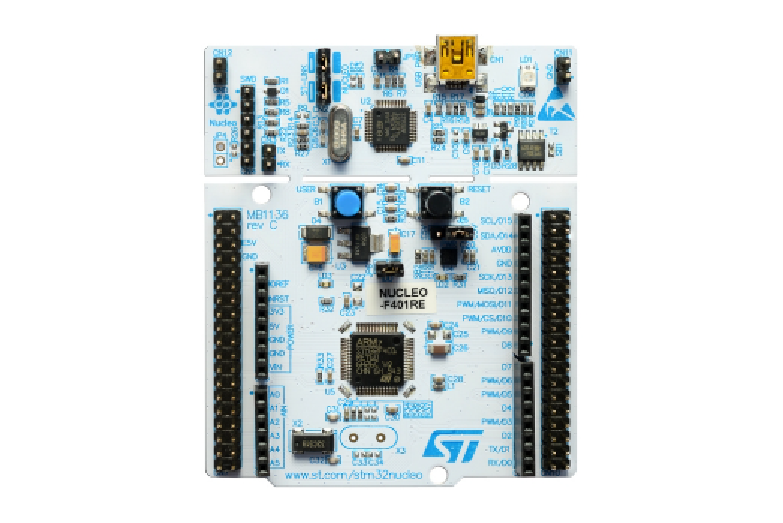
\includegraphics[width = 0.9\linewidth]{Figure/Board.pdf}
				\caption{Board NUCLEO STM32F4 F466RE}
			\end{figure}
			\begin{itemize}
				\item Specifications:
				\begin{itemize}
					\item STM32 microcontroller with LQFP64 package.
					\item Two types of extension resources
					\begin{itemize}
						\item Arduino Uno Revision 3 connectivity
						\item STMicroelectronics Morpho extension pin headers for full access to all STM32 I/Os
					\end{itemize}
					\item On-board ST-LINK/V2-1 debugger/programmer with SWD connector
					\begin{itemize}
						\item selection-mode switch to use the kit as a standalone ST-LINK/V2-1
					\end{itemize}
					\item Flexible board power supply
					\begin{itemize}
						\item USB VBUS or external source (3.3V, 5V, 7-12V)
						\item Power management access point
					\end{itemize}
					\item Three LEDs
					\begin{itemize}
						\item USB communication (LD1), user LED (LD2), power LED (LD3)
					\end{itemize}
					\item Two push buttons: USER and RESET
					\item USB re-enumeration capability: three different interfaces supported on USB
					\begin{itemize}
						\item Virtual Com port
						\item Mass storage
						\item Debug port
					\end{itemize}
					\item Supported by wide choice of Integrated Development Environments (IDEs) including $IAR^{TM}$, $Keil^{\circledR}$, GCC-based IDEs
				\end{itemize}
				\item Purpose: 
			\end{itemize}
		\subsection{Camera OV7670}
			\begin{figure}[!ht]
				\centering
				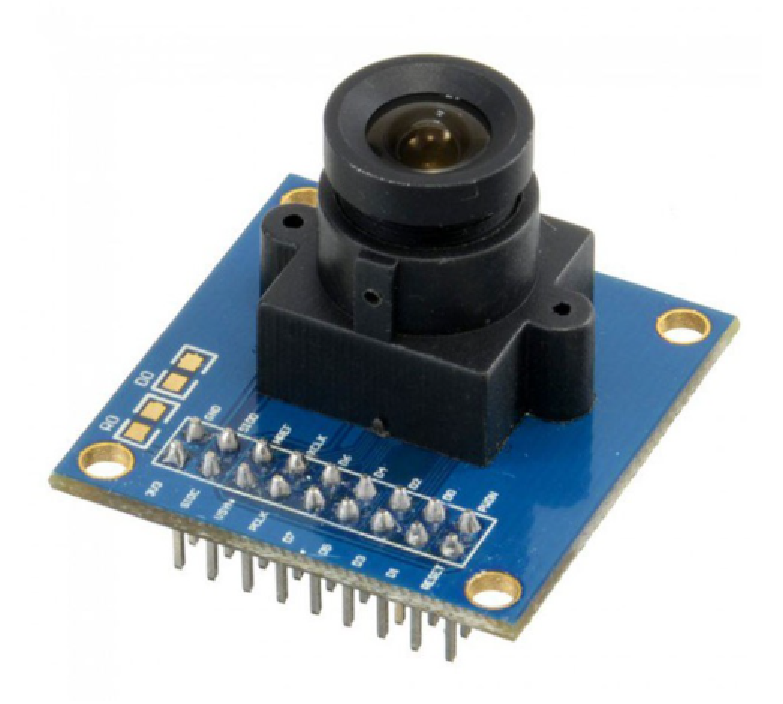
\includegraphics[width = 0.6\linewidth]{Figure/OV7670.pdf}
				\caption{Camera OV7670 no FIFO}
			\end{figure}
			\begin{itemize}
				\item Specifications:
				\begin{itemize}
					\item Photosensitive Array: 640x480
					\item IO Voltage: 2.5V to 3.0V
					\item Operating Power: 60mW/15fps
					\item Sleeping Mode: <20$\mu$A
					\item Operating Temperature: -30 to 70 deg C
					\item Output Format: YUV/YCbCr4:2:2 RGB565/555/444 GRB4:2:2 Raw RGB Data (8 digit)
					\item Lens Size: 1/6"
					\item Vision Angle: 25 degree
					\item Max Frame Rate: 30fps VGA
					\item Sensitivity: 1.3V / (lux-sec)
					\item Signal to Noise Ratio: 46dB
					\item DynamicRange: 52dB
					\item Browse Mode: By row
					\item Electronic Exposure: 1 to 510 row
					\item Pixel Coverage: 3.6$\mu$m x 3.6$\mu$m
					\item Duck Current: 12mV/s at 60 deg C
					\item PCB Size (L x W): Approx. 1.4x1.4inch / 3.5x3.5cm
				\end{itemize}
			\end{itemize}
		\newpage
		\subsection{Uart to MicroUSB CP2102}
			\begin{figure}[!ht]
				\centering
				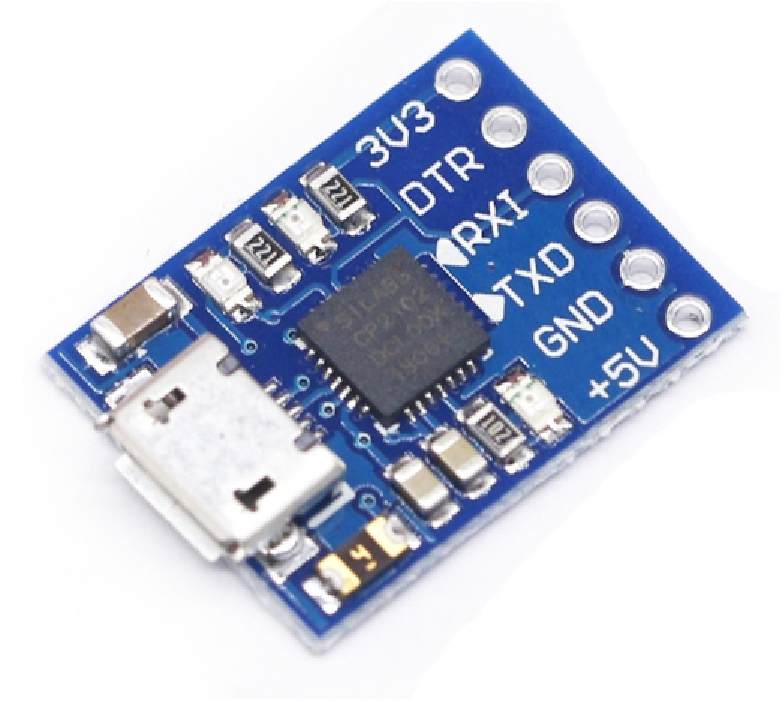
\includegraphics[width = 0.5\linewidth]{Figure/CP2102.pdf}
				\caption{UART to MicroUSB CP2102}
			\end{figure}
			\begin{itemize}
				\item Features:
					\begin{itemize}
						\item Embedded USB transceiver, no external circuit device
						\item Containing clock circuit, no external circuit device
						\item Contains power-on reset circuit
						\item The on-chip voltage regulator within the 3.3V output
						\item Meet the USB2.0 specification requirements
						\item SUSPEND pins support USB suspend state
						\item Asynchronous serial data bus compatible with all handshakes and modulation controller interface signals
						\item Support data format is 8 data bits, 1 stop bit and the parity bit
						\item Connotation 512 byte receive buffer and 512 byte transmit buffer
						\item Supports hardware or X-ON / X-OFF Handshake
						\item Size: 21x16mm
					\end{itemize}
			\end{itemize}
	\end{otherlanguage}
\end{document}